\begin{tikzpicture}
\pgfdeclareplotmark{cross} {
\pgfpathmoveto{\pgfpoint{-0.3\pgfplotmarksize}{\pgfplotmarksize}}
\pgfpathlineto{\pgfpoint{+0.3\pgfplotmarksize}{\pgfplotmarksize}}
\pgfpathlineto{\pgfpoint{+0.3\pgfplotmarksize}{0.3\pgfplotmarksize}}
\pgfpathlineto{\pgfpoint{+1\pgfplotmarksize}{0.3\pgfplotmarksize}}
\pgfpathlineto{\pgfpoint{+1\pgfplotmarksize}{-0.3\pgfplotmarksize}}
\pgfpathlineto{\pgfpoint{+0.3\pgfplotmarksize}{-0.3\pgfplotmarksize}}
\pgfpathlineto{\pgfpoint{+0.3\pgfplotmarksize}{-1.\pgfplotmarksize}}
\pgfpathlineto{\pgfpoint{-0.3\pgfplotmarksize}{-1.\pgfplotmarksize}}
\pgfpathlineto{\pgfpoint{-0.3\pgfplotmarksize}{-0.3\pgfplotmarksize}}
\pgfpathlineto{\pgfpoint{-1.\pgfplotmarksize}{-0.3\pgfplotmarksize}}
\pgfpathlineto{\pgfpoint{-1.\pgfplotmarksize}{0.3\pgfplotmarksize}}
\pgfpathlineto{\pgfpoint{-0.3\pgfplotmarksize}{0.3\pgfplotmarksize}}
\pgfpathclose
\pgfusepathqstroke
}
\pgfdeclareplotmark{cross*} {
\pgfpathmoveto{\pgfpoint{-0.3\pgfplotmarksize}{\pgfplotmarksize}}
\pgfpathlineto{\pgfpoint{+0.3\pgfplotmarksize}{\pgfplotmarksize}}
\pgfpathlineto{\pgfpoint{+0.3\pgfplotmarksize}{0.3\pgfplotmarksize}}
\pgfpathlineto{\pgfpoint{+1\pgfplotmarksize}{0.3\pgfplotmarksize}}
\pgfpathlineto{\pgfpoint{+1\pgfplotmarksize}{-0.3\pgfplotmarksize}}
\pgfpathlineto{\pgfpoint{+0.3\pgfplotmarksize}{-0.3\pgfplotmarksize}}
\pgfpathlineto{\pgfpoint{+0.3\pgfplotmarksize}{-1.\pgfplotmarksize}}
\pgfpathlineto{\pgfpoint{-0.3\pgfplotmarksize}{-1.\pgfplotmarksize}}
\pgfpathlineto{\pgfpoint{-0.3\pgfplotmarksize}{-0.3\pgfplotmarksize}}
\pgfpathlineto{\pgfpoint{-1.\pgfplotmarksize}{-0.3\pgfplotmarksize}}
\pgfpathlineto{\pgfpoint{-1.\pgfplotmarksize}{0.3\pgfplotmarksize}}
\pgfpathlineto{\pgfpoint{-0.3\pgfplotmarksize}{0.3\pgfplotmarksize}}
\pgfpathclose
\pgfusepathqfillstroke
}
\pgfdeclareplotmark{newstar} {
\pgfpathmoveto{\pgfqpoint{0pt}{\pgfplotmarksize}}
\pgfpathlineto{\pgfqpointpolar{44}{0.5\pgfplotmarksize}}
\pgfpathlineto{\pgfqpointpolar{18}{\pgfplotmarksize}}
\pgfpathlineto{\pgfqpointpolar{-20}{0.5\pgfplotmarksize}}
\pgfpathlineto{\pgfqpointpolar{-54}{\pgfplotmarksize}}
\pgfpathlineto{\pgfqpointpolar{-90}{0.5\pgfplotmarksize}}
\pgfpathlineto{\pgfqpointpolar{234}{\pgfplotmarksize}}
\pgfpathlineto{\pgfqpointpolar{198}{0.5\pgfplotmarksize}}
\pgfpathlineto{\pgfqpointpolar{162}{\pgfplotmarksize}}
\pgfpathlineto{\pgfqpointpolar{134}{0.5\pgfplotmarksize}}
\pgfpathclose
\pgfusepathqstroke
}
\pgfdeclareplotmark{newstar*} {
\pgfpathmoveto{\pgfqpoint{0pt}{\pgfplotmarksize}}
\pgfpathlineto{\pgfqpointpolar{44}{0.5\pgfplotmarksize}}
\pgfpathlineto{\pgfqpointpolar{18}{\pgfplotmarksize}}
\pgfpathlineto{\pgfqpointpolar{-20}{0.5\pgfplotmarksize}}
\pgfpathlineto{\pgfqpointpolar{-54}{\pgfplotmarksize}}
\pgfpathlineto{\pgfqpointpolar{-90}{0.5\pgfplotmarksize}}
\pgfpathlineto{\pgfqpointpolar{234}{\pgfplotmarksize}}
\pgfpathlineto{\pgfqpointpolar{198}{0.5\pgfplotmarksize}}
\pgfpathlineto{\pgfqpointpolar{162}{\pgfplotmarksize}}
\pgfpathlineto{\pgfqpointpolar{134}{0.5\pgfplotmarksize}}
\pgfpathclose
\pgfusepathqfillstroke
}
\definecolor{c}{rgb}{1,1,1};
\draw [color=c, fill=c] (0,0) rectangle (20,14.3108);
\draw [color=c, fill=c] (3.2,2.28972) rectangle (19,13.5952);
\definecolor{c}{rgb}{0,0,0};
\draw [c,line width=0.9] (3.2,2.28972) -- (3.2,13.5952) -- (19,13.5952) -- (19,2.28972) -- (3.2,2.28972);
\definecolor{c}{rgb}{0.719608,0.263113,0.13652};
\draw [color=c, fill=c] (3.2,2.28972) rectangle (6.53333,4.40951);
\definecolor{c}{rgb}{0.817157,0.659804,0.345588};
\draw [color=c, fill=c] (6.53333,2.28972) rectangle (9.86667,4.40951);
\definecolor{c}{rgb}{0.851961,0.792892,0.499387};
\draw [color=c, fill=c] (9.86667,2.28972) rectangle (12.3333,4.40951);
\definecolor{c}{rgb}{0.842647,0.888358,0.743873};
\draw [color=c, fill=c] (13.3333,2.28972) rectangle (16.5333,4.40951);
\definecolor{c}{rgb}{0.864706,0.840686,0.58701};
\draw [color=c, fill=c] (16.5333,2.28972) rectangle (19,4.40951);
\definecolor{c}{rgb}{0.743137,0.361642,0.174755};
\draw [color=c, fill=c] (3.2,4.40951) rectangle (6.53333,5.8227);
\definecolor{c}{rgb}{0.851961,0.792892,0.499387};
\draw [color=c, fill=c] (6.53333,4.40951) rectangle (9.86667,5.8227);
\definecolor{c}{rgb}{0.860294,0.872181,0.670343};
\draw [color=c, fill=c] (9.86667,4.40951) rectangle (12.3333,5.8227);
\draw [color=c, fill=c] (13.3333,4.40951) rectangle (16.5333,5.8227);
\definecolor{c}{rgb}{0.864706,0.840686,0.58701};
\draw [color=c, fill=c] (16.5333,4.40951) rectangle (19,5.8227);
\definecolor{c}{rgb}{0.743137,0.361642,0.174755};
\draw [color=c, fill=c] (3.2,5.8227) rectangle (6.53333,7.94248);
\definecolor{c}{rgb}{0.851961,0.792892,0.499387};
\draw [color=c, fill=c] (6.53333,5.8227) rectangle (9.86667,7.94248);
\definecolor{c}{rgb}{0.860294,0.872181,0.670343};
\draw [color=c, fill=c] (9.86667,5.8227) rectangle (12.3333,7.94248);
\definecolor{c}{rgb}{0.842647,0.888358,0.743873};
\draw [color=c, fill=c] (13.3333,5.8227) rectangle (16.5333,7.94248);
\definecolor{c}{rgb}{0.860294,0.872181,0.670343};
\draw [color=c, fill=c] (16.5333,5.8227) rectangle (19,7.94248);
\definecolor{c}{rgb}{0.817157,0.659804,0.345588};
\draw [color=c, fill=c] (3.2,7.94248) rectangle (6.53333,13.5952);
\definecolor{c}{rgb}{0.864706,0.840686,0.58701};
\draw [color=c, fill=c] (6.53333,7.94248) rectangle (9.86667,13.5952);
\definecolor{c}{rgb}{0.860294,0.872181,0.670343};
\draw [color=c, fill=c] (9.86667,7.94248) rectangle (12.3333,13.5952);
\definecolor{c}{rgb}{0.842647,0.888358,0.743873};
\draw [color=c, fill=c] (13.3333,7.94248) rectangle (16.5333,13.5952);
\definecolor{c}{rgb}{0.860294,0.872181,0.670343};
\draw [color=c, fill=c] (16.5333,7.94248) rectangle (19,13.5952);
\definecolor{c}{rgb}{0,0,0};
\draw (4.86667,3.34962) node[scale=1.61424, color=c, rotate=1]{$\genfrac{}{}{0pt}{}{1.63}{\pm 0.05}$};
\draw (8.2,3.34962) node[scale=1.61424, color=c, rotate=1]{$\genfrac{}{}{0pt}{}{1.28}{\pm 0.03}$};
\draw (11.1,3.34962) node[scale=1.61424, color=c, rotate=1]{$\genfrac{}{}{0pt}{}{1.09}{\pm 0.02}$};
\draw (14.9333,3.34962) node[scale=1.61424, color=c, rotate=1]{$\genfrac{}{}{0pt}{}{0.87}{\pm 0.02}$};
\draw (17.7667,3.34962) node[scale=1.61424, color=c, rotate=1]{$\genfrac{}{}{0pt}{}{1.04}{\pm 0.01}$};
\draw (4.86667,5.1161) node[scale=1.61424, color=c, rotate=1]{$\genfrac{}{}{0pt}{}{1.49}{\pm 0.02}$};
\draw (8.2,5.1161) node[scale=1.61424, color=c, rotate=1]{$\genfrac{}{}{0pt}{}{1.12}{\pm 0.02}$};
\draw (11.1,5.1161) node[scale=1.61424, color=c, rotate=1]{$\genfrac{}{}{0pt}{}{0.93}{\pm 0.01}$};
\draw (14.9333,5.1161) node[scale=1.61424, color=c, rotate=1]{$\genfrac{}{}{0pt}{}{0.90}{\pm 0.01}$};
\draw (17.7667,5.1161) node[scale=1.61424, color=c, rotate=1]{$\genfrac{}{}{0pt}{}{1.00}{\pm 0.01}$};
\draw (4.86667,6.88259) node[scale=1.61424, color=c, rotate=1]{$\genfrac{}{}{0pt}{}{1.48}{\pm 0.03}$};
\draw (8.2,6.88259) node[scale=1.61424, color=c, rotate=1]{$\genfrac{}{}{0pt}{}{1.08}{\pm 0.02}$};
\draw (11.1,6.88259) node[scale=1.61424, color=c, rotate=1]{$\genfrac{}{}{0pt}{}{0.92}{\pm 0.02}$};
\draw (14.9333,6.88259) node[scale=1.61424, color=c, rotate=1]{$\genfrac{}{}{0pt}{}{0.89}{\pm 0.01}$};
\draw (17.7667,6.88259) node[scale=1.61424, color=c, rotate=1]{$\genfrac{}{}{0pt}{}{0.95}{\pm 0.01}$};
\draw (4.86667,10.7689) node[scale=1.61424, color=c, rotate=1]{$\genfrac{}{}{0pt}{}{1.24}{\pm 0.15}$};
\draw (8.2,10.7689) node[scale=1.61424, color=c, rotate=1]{$\genfrac{}{}{0pt}{}{1.02}{\pm 0.08}$};
\draw (11.1,10.7689) node[scale=1.61424, color=c, rotate=1]{$\genfrac{}{}{0pt}{}{0.95}{\pm 0.07}$};
\draw (14.9333,10.7689) node[scale=1.61424, color=c, rotate=1]{$\genfrac{}{}{0pt}{}{0.90}{\pm 0.05}$};
\draw (17.7667,10.7689) node[scale=1.61424, color=c, rotate=1]{$\genfrac{}{}{0pt}{}{0.97}{\pm 0.05}$};
\draw [c,line width=0.9] (3.2,2.28972) -- (19,2.28972);
\draw [anchor=north] (4.86667,2.12014) node[scale=1.0576, color=c, rotate=0]{[0.0 - 0.5]};
\draw [anchor=north] (8.2,2.12014) node[scale=1.0576, color=c, rotate=0]{[0.5 - 1.0]};
\draw [anchor=north] (11.1,2.12014) node[scale=1.0576, color=c, rotate=0]{[1.0 - 1.37]};
% \draw [anchor=north] (12.8333,2.12014) node[scale=1.0576, color=c, rotate=0]{[1.37 - 1.52]};
\draw [anchor=north] (14.9333,2.12014) node[scale=1.0576, color=c, rotate=0]{[1.52 - 2.0]};
\draw [anchor=north] (17.7667,2.12014) node[scale=1.0576, color=c, rotate=0]{[2.0 - 2.37]};
\draw [c,line width=0.9] (3.2,2.62889) -- (3.2,2.28972);
\draw [c,line width=0.9] (6.53333,2.62889) -- (6.53333,2.28972);
\draw [c,line width=0.9] (9.86667,2.62889) -- (9.86667,2.28972);
\draw [c,line width=0.9] (13.2,2.62889) -- (13.2,2.28972);
\draw [c,line width=0.9] (16.5333,2.62889) -- (16.5333,2.28972);
\draw [c,line width=0.9] (16.5333,2.62889) -- (16.5333,2.28972);
\draw [anchor= east] (19,0.686917) node[scale=1.61424, color=c, rotate=0]{$|\eta|_{  e/\gamma}^{probe}$};
\draw [c,line width=0.9] (3.2,13.5952) -- (19,13.5952);
\draw [c,line width=0.9] (3.2,13.2561) -- (3.2,13.5952);
\draw [c,line width=0.9] (6.53333,13.2561) -- (6.53333,13.5952);
\draw [c,line width=0.9] (9.86667,13.2561) -- (9.86667,13.5952);
\draw [c,line width=0.9] (13.2,13.2561) -- (13.2,13.5952);
\draw [c,line width=0.9] (16.5333,13.2561) -- (16.5333,13.5952);
\draw [c,line width=0.9] (16.5333,13.2561) -- (16.5333,13.5952);
\draw [c,line width=0.9] (3.2,2.28972) -- (3.2,13.5952);
\draw [anchor= east] (2.963,3.34962) node[scale=1.0576, color=c, rotate=0]{[20 - 35] };
\draw [anchor= east] (2.963,5.1161) node[scale=1.0576, color=c, rotate=0]{[35 - 45] };
\draw [anchor= east] (2.963,6.88259) node[scale=1.0576, color=c, rotate=0]{[45 - 60] };
\draw [anchor= east] (2.963,8.6) node[scale=1.0576, color=c, rotate=0]{[60 - 100]};
\draw [c,line width=0.9] (3.674,2.28972) -- (3.2,2.28972);
\draw [c,line width=0.9] (3.674,5.1161) -- (3.2,5.1161);
\draw [c,line width=0.9] (3.674,7.94248) -- (3.2,7.94248);
\draw [c,line width=0.9] (3.674,10.7689) -- (3.2,10.7689);
\draw [c,line width=0.9] (3.674,13.5952) -- (3.2,13.5952);
\draw [anchor= east] (0.96,13.5952) node[scale=1.61424, color=c, rotate=90]{$p_{T,  e/\gamma}^{probe}  [GeV]$};
\draw [c,line width=0.9] (19,2.28972) -- (19,13.5952);
\draw [c,line width=0.9] (18.526,2.28972) -- (19,2.28972);
\draw [c,line width=0.9] (18.526,5.1161) -- (19,5.1161);
\draw [c,line width=0.9] (18.526,7.94248) -- (19,7.94248);
\draw [c,line width=0.9] (18.526,10.7689) -- (19,10.7689);
\draw [c,line width=0.9] (18.526,13.5952) -- (19,13.5952);
\definecolor{c}{rgb}{0.18229,0.273751,0.887287};
\draw [color=c, fill=c] (19.1,2.28972) rectangle (19.99,2.855);
\definecolor{c}{rgb}{0.248071,0.40038,0.854396};
\draw [color=c, fill=c] (19.1,2.855) rectangle (19.99,3.42028);
\definecolor{c}{rgb}{0.323039,0.505147,0.851225};
\draw [color=c, fill=c] (19.1,3.42028) rectangle (19.99,3.98555);
\definecolor{c}{rgb}{0.39951,0.584559,0.871814};
\draw [color=c, fill=c] (19.1,3.98555) rectangle (19.99,4.55083);
\definecolor{c}{rgb}{0.482353,0.670588,0.894118};
\draw [color=c, fill=c] (19.1,4.55083) rectangle (19.99,5.1161);
\definecolor{c}{rgb}{0.541299,0.734314,0.884559};
\draw [color=c, fill=c] (19.1,5.1161) rectangle (19.99,5.68138);
\definecolor{c}{rgb}{0.600245,0.798039,0.875};
\draw [color=c, fill=c] (19.1,5.68138) rectangle (19.99,6.24665);
\definecolor{c}{rgb}{0.664216,0.842157,0.861765};
\draw [color=c, fill=c] (19.1,6.24665) rectangle (19.99,6.81193);
\definecolor{c}{rgb}{0.743873,0.87402,0.842647};
\draw [color=c, fill=c] (19.1,6.81193) rectangle (19.99,7.37721);
\definecolor{c}{rgb}{0.823529,0.905882,0.823529};
\draw [color=c, fill=c] (19.1,7.37721) rectangle (19.99,7.94248);
\definecolor{c}{rgb}{0.842647,0.888358,0.743873};
\draw [color=c, fill=c] (19.1,7.94248) rectangle (19.99,8.50776);
\definecolor{c}{rgb}{0.860294,0.872181,0.670343};
\draw [color=c, fill=c] (19.1,8.50776) rectangle (19.99,9.07303);
\definecolor{c}{rgb}{0.864706,0.840686,0.58701};
\draw [color=c, fill=c] (19.1,9.07303) rectangle (19.99,9.63831);
\definecolor{c}{rgb}{0.851961,0.792892,0.499387};
\draw [color=c, fill=c] (19.1,9.63831) rectangle (19.99,10.2036);
\definecolor{c}{rgb}{0.839216,0.745098,0.411765};
\draw [color=c, fill=c] (19.1,10.2036) rectangle (19.99,10.7689);
\definecolor{c}{rgb}{0.817157,0.659804,0.345588};
\draw [color=c, fill=c] (19.1,10.7689) rectangle (19.99,11.3341);
\definecolor{c}{rgb}{0.79326,0.567402,0.273897};
\draw [color=c, fill=c] (19.1,11.3341) rectangle (19.99,11.8994);
\definecolor{c}{rgb}{0.768627,0.468382,0.216176};
\draw [color=c, fill=c] (19.1,11.8994) rectangle (19.99,12.4647);
\definecolor{c}{rgb}{0.743137,0.361642,0.174755};
\draw [color=c, fill=c] (19.1,12.4647) rectangle (19.99,13.03);
\definecolor{c}{rgb}{0.719608,0.263113,0.13652};
\draw [color=c, fill=c] (19.1,13.03) rectangle (19.99,13.5952);
\definecolor{c}{rgb}{0,0,0};
\draw [c,line width=0.9] (19.99,2.28972) -- (19.99,13.5952);
\draw [c,line width=0.9] (19.516,2.28972) -- (19.99,2.28972);
\draw [c,line width=0.9] (19.516,3.67308) -- (19.99,3.67308);
\draw [c,line width=0.9] (19.516,5.05644) -- (19.99,5.05644);
\draw [c,line width=0.9] (19.516,6.4398) -- (19.99,6.4398);
\draw [c,line width=0.9] (19.516,7.82315) -- (19.99,7.82315);
\draw [c,line width=0.9] (19.516,9.20651) -- (19.99,9.20651);
\draw [c,line width=0.9] (19.516,10.5899) -- (19.99,10.5899);
\draw [c,line width=0.9] (19.516,11.9732) -- (19.99,11.9732);
\draw [c,line width=0.9] (19.516,13.3566) -- (19.99,13.3566);
\draw [c,line width=0.9] (19.516,13.3566) -- (19.99,13.3566);
\draw [anchor= west] (20.09,2.28972) node[scale=1.61424, color=c, rotate=0]{0};
\draw [anchor= west] (20.09,3.67308) node[scale=1.61424, color=c, rotate=0]{0.2};
\draw [anchor= west] (20.09,5.05644) node[scale=1.61424, color=c, rotate=0]{0.4};
\draw [anchor= west] (20.09,6.4398) node[scale=1.61424, color=c, rotate=0]{0.6};
\draw [anchor= west] (20.09,7.82315) node[scale=1.61424, color=c, rotate=0]{0.8};
\draw [anchor= west] (20.09,9.20651) node[scale=1.61424, color=c, rotate=0]{1};
\draw [anchor= west] (20.09,10.5899) node[scale=1.61424, color=c, rotate=0]{1.2};
\draw [anchor= west] (20.09,11.9732) node[scale=1.61424, color=c, rotate=0]{1.4};
\draw [anchor= west] (20.09,13.3566) node[scale=1.61424, color=c, rotate=0]{1.6};
\end{tikzpicture}
